\documentclass{article}

% if you need to pass options to natbib, use, e.g.:
%     \PassOptionsToPackage{numbers, compress}{natbib}
% before loading neurips_2026

% Submission/track options (see neurips_2026.sty header).
% We use the "preprint" track so author identity is shown, line numbers
% are removed, and the footer reads "Preprint. Work in progress." which
% is appropriate for a graded course report rather than a blind review.
\usepackage[preprint]{neurips_2026}

\usepackage[utf8]{inputenc}
\usepackage[T1]{fontenc}
\usepackage{hyperref}
\usepackage{url}
\usepackage{booktabs}
\usepackage{amsfonts}
\usepackage{amsmath}
\usepackage{amssymb}
\usepackage{nicefrac}
\usepackage{microtype}
\usepackage{xcolor}
\usepackage{graphicx}
\usepackage{tikz}
\usetikzlibrary{positioning, arrows.meta, shapes.geometric, fit, backgrounds, calc}
\usepackage{multirow}
\usepackage{caption}
\usepackage{subcaption}
\captionsetup{font=small, labelfont=bf}
\graphicspath{{figures/}}

\title{Re-Implementing CNN Price-Trend Signals:\\
A Reproduction of Jiang, Kelly, and Xiu (2023)}

\author{%
  Kaibiao Zhu \\
  Final Project, Machine Learning for Finance \\
  The Hong Kong University of Science and Technology (Guangzhou) \\
  \texttt{kzhu597@connect.hkust-gz.edu.cn}
}


\begin{document}


\maketitle


\begin{abstract}
This paper reproduces the image-based price-trend prediction framework of
\citet{jiang2023reimagining}, which replaces predefined technical indicators
with OHLC-volume charts and convolutional neural networks (CNNs). Using CRSP
daily U.S. equity data, we reconstruct the image pipeline, train horizon-specific
CNN ensembles, and evaluate the resulting signals through out-of-sample backtests. We compare the CNN signals with momentum,
moving-average, and reversal benchmarks, and assess residual performance through
factor-spanning regressions. The reproduction is strongest at short horizons,
where image-based signals deliver the best economic performance. Relative to
the magnitudes reported by \citet{jiang2023reimagining}, medium- and
long-horizon strategies weaken substantially after costs, and factor stripping
yields significantly negative alphas. Saliency
maps indicate that the CNN mainly attends to recent price movement and volume
contrast. We release all code and artefacts needed to audit and extend the
reproduction.
\end{abstract}


\section{Introduction}
\label{sec:intro}

Technical analysis has long suggested that the visual ``shape'' of a price
chart conveys information beyond what is captured by scalar momentum or
moving-average filters. \citet{jiang2023reimagining} formalise this intuition
by feeding fixed-resolution open--high--low--close (OHLC) images with a
volume sub-panel into a convolutional neural network and showing that the
resulting forecasts dominate canonical price-trend signals out of sample.
Their work joins a growing empirical asset-pricing literature that uses
flexible machine-learning predictors to map raw historical features into
expected returns \citep{gu2020empirical,kelly2019characteristics}, and it
ties directly to early efforts at formalising chart patterns via kernel
smoothing \citep{lo2000foundations}.

This paper re-implements the core pipeline from end to end and evaluates it
under the same in-sample and out-of-sample calendar design as
\citet{jiang2023reimagining}: training and validation draw from 1993--2000
with a 70/30 random sample split, and headline out-of-sample results are
reported for 2001--2019. Our contributions are:
\begin{enumerate}
  \item An independent OHLC-plus-volume image renderer and horizon-matched CNN
        stacks built from the dimensions, drawing rules, and layer geometry
        documented in \citet{jiang2023reimagining}---including the simple
        moving-average overlay, volume sub-panel, and vertical orientation
        convention---implemented from the paper's written specification and
        reported tensor dimensions.
  \item A CRSP-style daily panel spanning 1992--2024 for data construction, with
        out-of-sample CNN evaluation for 2001--2019 as above; proportional transaction
        costs; matched-horizon price momentum, simple moving-average cross,
        and short-term reversal baselines; and a five-factor-plus-momentum
        spanning regression \citep{fama1993common,fama2015five,carhart1997persistence}.
  \item Input-gradient saliency analysis \citep{simonyan2014deep} of the
        $I=60$ ensemble, which highlights the right tail of each image and
        the volume bars as the dominant feature regions.
  \item Public release of code, trained weights, and post-aggregation CSV
        tables in \texttt{final\_submit\_version/}, allowing every numerical
        claim to be regenerated.
\end{enumerate}

The remainder of the paper is organised as follows. Section~\ref{sec:related}
positions our reproduction relative to the chart-pattern, deep-learning, and
interpretability literatures. Section~\ref{sec:data} details data sources and
image construction. Section~\ref{sec:arch} describes the CNN architecture and
training recipe. Section~\ref{sec:results} reports empirical results
(decile prediction accuracy, baseline comparisons, cumulative returns,
classification metrics, decile portfolio statistics, and Fama--French
spanning regressions). Section~\ref{sec:saliency} visualises model
attention. Section~\ref{sec:discussion} discusses where our results align
with and diverge from \citet{jiang2023reimagining}.


\section{Related work}
\label{sec:related}

\paragraph{Chart-pattern literature.}
\citet{lo2000foundations} provided one of the first systematic treatments
of technical chart patterns by combining kernel regression with automated
pattern recognition. \citet{jegadeesh1993returns} documented price momentum
as a robust cross-sectional return predictor, providing the canonical
benchmark against which any technical-trend signal must be compared.

\paragraph{Deep learning for return prediction.}
Recent work demonstrates that deep architectures uncover return signals
that are difficult to capture with closed-form characteristics. \citet{gu2020empirical}
benchmark a broad set of supervised learners on U.S. equities;
\citet{kelly2019characteristics} use latent-factor models with characteristic
loadings. Within technical analysis, \citet{sezer2018algorithmic} convert
indicators into images for trading. \citet{jiang2023reimagining} unify these
threads by treating the OHLC chart itself as the model input.

\paragraph{Interpretability via input gradients.}
\citet{simonyan2014deep} introduced gradient-based saliency to visualise
which input pixels most influence a CNN's class score; we apply the same
technique to identify which segments of each OHLC image drive the model's
``up'' probability. CNN architectures used here trace back to
\citet{lecun1998gradient}.


\section{Data and image construction}
\label{sec:data}

\paragraph{Universe.}
We use a CRSP-style daily equity panel covering 1992-01-01 to 2024-12-31.
The cleaning step retains the following columns per
\texttt{final\_submit\_version/docs/variable\_description.txt}:
\texttt{permno}, \texttt{dlycaldt}, \texttt{dlycap}, \texttt{dlyret},
\texttt{dlyretx}, \texttt{dlyvol}, \texttt{dlyopen}, \texttt{dlyhigh},
\texttt{dlylow}, \texttt{dlyclose}. We drop rows with any of those columns
missing, apply a $\$1$ minimum-close and strictly positive
volume filter, and compute log returns and adjusted OHLC prices via
cumulative log-return compounding so that the first valid observation per
\texttt{permno} acts as the price anchor. No survivorship adjustments are
applied beyond what is implicit in the CRSP-style file.

\paragraph{Labels and holding period.}
For each horizon $F\in\{5,20,60\}$ trading days we form
$R^{\mathrm{fut}}_{t,F}=\exp\!\bigl(\sum_{s=t+1}^{t+F}\log(1+r_s)\bigr)-1$ on
the adjusted price path, and a binary classification label
$y_{t,F}=\mathbb{1}\{R^{\mathrm{fut}}_{t,F}>0\}$. Rebalance timestamps are
fixed at period-end calendar boundaries (Friday for $F=5$, month-end for
$F=20$, quarter-end for $F=60$), matching the canonical SPY trade calendar.

\paragraph{Image construction.}
For input horizon $I\in\{5,20,60\}$ matched to $F=I$ we render a grayscale
image of width $W=3I$ and height $H$ split into an OHLC panel of height
$H_{\mathrm{ohlc}}$ stacked above a one-pixel-gap volume panel of height
$H_{\mathrm{vol}}$:
\begin{center}
  \begin{tabular}{cccc}
    \toprule
    Horizon & $W$ & $H_{\mathrm{ohlc}}$ & $H_{\mathrm{vol}}$ \\
    \midrule
    $I=5$  & 15  & 25 & 6  \\
    $I=20$ & 60  & 51 & 12 \\
    $I=60$ & 180 & 76 & 19 \\
    \bottomrule
  \end{tabular}
\end{center}
For each day $\tau$ in the window we draw (a) a one-pixel vertical bar from
the low to the high, (b) a one-pixel open tick at column $3\tau$ and a
close tick at column $3\tau+2$, (c) a one-pixel SMA poly-line connecting
the rolling $I$-day means of close prices (computed using $2I-1$ days of
history so that the first SMA point already reflects $I$ observations),
all scaled to a common $[P_{\min},P_{\max}]$ range that includes the SMA
values. Volume bars are normalised to the window's own maximum. The
finished OHLC panel is finally flipped top-to-bottom so that ``up'' moves
appear visually upward, then concatenated with the volume panel with a
one-pixel gap. Figure~\ref{fig:ohlc-sample} shows the three resolutions
for a single \texttt{permno} anchored at the same calendar date.

\begin{figure}[t]
  \centering
  
\includegraphics[width=\linewidth]{ohlc_sample.png}
  \caption{OHLC-plus-volume images for a single security at horizons
    $I\in\{5,20,60\}$. The same calendar anchor (2010-12-31) is used so
    the visual density at different resolutions is directly comparable.}
  \label{fig:ohlc-sample}
\end{figure}

\paragraph{Train/validation/test split.}
We follow \citet{jiang2023reimagining} in treating the early portion of
the panel as in-sample. Training is performed on 1993--2000 with a
70/30 random sample-level split for training/validation. Out-of-sample
backtests start in 2001 and run through to the end of the cached panel.
For the headline tables and figures we report results from 2001-01 to
2019-12 to align with where all baseline ETFs (used for calendar
construction) have continuous coverage.


\section{CNN architecture and training}
\label{sec:arch}

\paragraph{Architectures.}
The three horizon-specific backbones mirror the published configuration.
All blocks use $5\times3$ kernels, a LeakyReLU($0.01$) activation, batch
normalisation, and $(2,1)$ MaxPool with \texttt{ceil\_mode=True} (the $I=5$
head uses the standard floor mode). $I=20$ and $I=60$ insert dilated and
strided first convolutions so the receptive field can span longer windows
without an explosion in parameter count. Figure~\ref{fig:cnn-arch}
summarises the three stacks; layer-level details are in
Table~\ref{tab:cnn-layers} (Appendix~\ref{app:hyper}).

\begin{figure}[t]
  \centering
  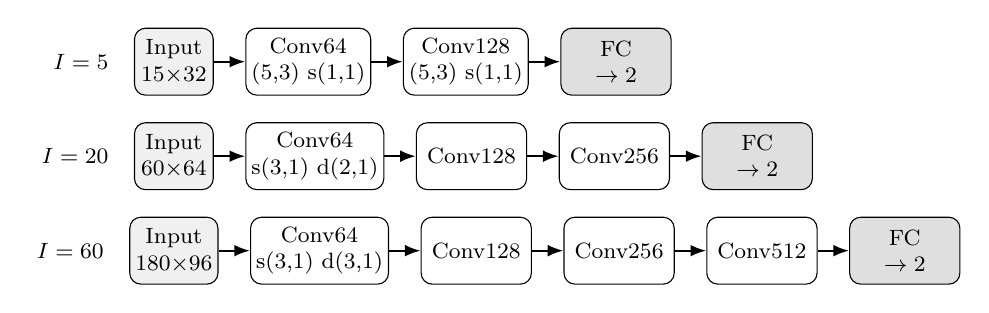
\begin{tikzpicture}[
      font=\footnotesize,
      block/.style={draw, rounded corners, minimum height=0.85cm, minimum width=1.4cm, align=center, inner sep=2pt},
      input/.style={draw, fill=gray!12, rounded corners, minimum height=0.85cm, minimum width=1.0cm, align=center, inner sep=2pt},
      head/.style={draw, fill=gray!25, rounded corners, minimum height=0.85cm, minimum width=1.4cm, align=center, inner sep=2pt},
      arr/.style={-{Latex[length=2mm]}, thick}
    ]
    %% I=5 row
    \node[input] (i5in) at (0,2.2) {Input\\$15{\times}32$};
    \node[block, right=4mm of i5in] (i5b1) {Conv64\\(5,3) s(1,1)};
    \node[block, right=4mm of i5b1] (i5b2) {Conv128\\(5,3) s(1,1)};
    \node[head,  right=4mm of i5b2] (i5fc) {FC\\$\to 2$};
    \draw[arr] (i5in)  -- (i5b1);
    \draw[arr] (i5b1)  -- (i5b2);
    \draw[arr] (i5b2)  -- (i5fc);
    \node[left=2mm of i5in] {$I=5$};
    %% I=20 row
    \node[input] (i20in) at (0,1.0) {Input\\$60{\times}64$};
    \node[block, right=4mm of i20in] (i20b1) {Conv64\\s(3,1) d(2,1)};
    \node[block, right=4mm of i20b1] (i20b2) {Conv128};
    \node[block, right=4mm of i20b2] (i20b3) {Conv256};
    \node[head,  right=4mm of i20b3] (i20fc) {FC\\$\to 2$};
    \draw[arr] (i20in) -- (i20b1);
    \draw[arr] (i20b1) -- (i20b2);
    \draw[arr] (i20b2) -- (i20b3);
    \draw[arr] (i20b3) -- (i20fc);
    \node[left=2mm of i20in] {$I=20$};
    %% I=60 row
    \node[input] (i60in) at (0,-0.2) {Input\\$180{\times}96$};
    \node[block, right=4mm of i60in] (i60b1) {Conv64\\s(3,1) d(3,1)};
    \node[block, right=4mm of i60b1] (i60b2) {Conv128};
    \node[block, right=4mm of i60b2] (i60b3) {Conv256};
    \node[block, right=4mm of i60b3] (i60b4) {Conv512};
    \node[head,  right=4mm of i60b4] (i60fc) {FC\\$\to 2$};
    \draw[arr] (i60in) -- (i60b1);
    \draw[arr] (i60b1) -- (i60b2);
    \draw[arr] (i60b2) -- (i60b3);
    \draw[arr] (i60b3) -- (i60b4);
    \draw[arr] (i60b4) -- (i60fc);
    \node[left=2mm of i60in] {$I=60$};
  \end{tikzpicture}
  \caption{Horizon-specific CNN backbones. Each rectangle represents one
    Conv$\to$BatchNorm$\to$LeakyReLU$\to$MaxPool block. All kernels are
    $5\times 3$; default stride and dilation are $(1,1)$ except where
    explicitly noted. The fully-connected head has dropout $0.5$ and
    outputs two logits.}
  \label{fig:cnn-arch}
\end{figure}

\paragraph{Optimisation.}
We minimise binary cross-entropy on the per-horizon label $y_{t,F}$ using
stochastic gradient descent (Adam variant disabled), with learning rate
$10^{-5}$, batch size $128$, and a maximum of $50$ epochs with
early-stopping on validation loss. Convolutional and linear weights are
initialised with Xavier-uniform and biases at zero. We train an ensemble
of five seeds $\{42, 123, 456, 789, 101112\}$ and aggregate by averaging
the softmax-probability outputs at inference time. The resulting
checkpoints are stored under
\texttt{final\_submit\_version/outputs/models/} with sizes $\approx
0.6$\,MB ($I=5$), $\approx 2.8$\,MB ($I=20$), and $\approx 11.8$\,MB
($I=60$) per seed, consistent with the parameter counts implied by
Figure~\ref{fig:cnn-arch}.


\section{Empirical results}
\label{sec:results}

We score every test-set observation with the five-seed ensemble and
form ten cross-sectional deciles by predicted ``up''-probability at each
rebalance date. The high-minus-low (H--L) portfolio is equal-weighted
within deciles, rebalanced at horizon-end, and adjusted for proportional
transaction costs at $10$\,bp per side ($20$\,bp round-trip) applied to
both legs.

\subsection{Decile prediction accuracy (Figure 6 reproduction)}
\label{sec:r1}

\begin{figure}[t]
  \centering
  \begin{subfigure}[t]{0.32\linewidth}\centering
    
\includegraphics[width=\linewidth]{fig6_I5.png}
    \caption{$I=5$}
  \end{subfigure}\hfill
  \begin{subfigure}[t]{0.32\linewidth}\centering
    
\includegraphics[width=\linewidth]{fig6_I20.png}
    \caption{$I=20$}
  \end{subfigure}\hfill
  \begin{subfigure}[t]{0.32\linewidth}\centering
    
\includegraphics[width=\linewidth]{fig6_I60.png}
    \caption{$I=60$}
  \end{subfigure}
  \caption{Annualised decile returns by horizon for the CNN, matched-horizon
    momentum, and moving-average cross signals. Reproduction of Figure~6 of
    \citet{jiang2023reimagining}. Numbers are read from
    \texttt{outputs/pipeline\_runs/tables/fig6\_I\{5,20,60\}\_\{cnn,mom,ma\}.csv}.}
  \label{fig:fig6}
\end{figure}

At $I=5$ the CNN decile annualised returns rise nearly monotonically from
$6.62\%$ in D1 to $20.67\%$ in D10 (Figure~\ref{fig:fig6}a), while the
five-day momentum and moving-average curves are essentially flat across
the cross-section. At longer horizons the picture changes: the $I=20$
CNN spread between D10 and D1 is mildly positive ($11.10\%$ vs.\ $9.78\%$;
Figure~\ref{fig:fig6}b), and at $I=60$ the CNN ordering is essentially
flat ($11.95\%$ in D10 against $13.00\%$ in D1; Figure~\ref{fig:fig6}c).
The traditional baselines, by contrast, display a U-shaped pattern at
$I=20$ and $I=60$: both the bottom and top deciles deliver above-average
returns, reflecting the well-known concentration of momentum and
mean-reversion premia in the extreme deciles.

\subsection{Comparison with traditional baselines (Figure 7)}

\begin{figure}[t]
  \centering
  \begin{subfigure}[t]{0.32\linewidth}\centering
    
\includegraphics[width=\linewidth]{fig7_I5.png}
    \caption{$I=5$}
  \end{subfigure}\hfill
  \begin{subfigure}[t]{0.32\linewidth}\centering
    
\includegraphics[width=\linewidth]{fig7_I20.png}
    \caption{$I=20$}
  \end{subfigure}\hfill
  \begin{subfigure}[t]{0.32\linewidth}\centering
    
\includegraphics[width=\linewidth]{fig7_I60.png}
    \caption{$I=60$}
  \end{subfigure}
  \caption{Simplified Figure~7 reproduction: CNN deciles against momentum,
    moving-average cross, and short-term reversal baselines. At $I=5$ the
    reversal baseline's D10 reaches an annualised return of $37.78\%$,
    against which the CNN's monotone ranking is more useful as a signal
    than as a stand-alone strategy.}
  \label{fig:fig7}
\end{figure}

Figure~\ref{fig:fig7} shows that at $I=5$ the CNN ranking strictly
dominates both momentum and moving-average cross across the cross-section,
but is itself dominated in absolute level by the short-term reversal
baseline whose D10 annualised return reaches $37.78\%$ (driven by the
microstructure-style bid--ask bounce on which it relies). At $I=20$ the
momentum and moving-average curves display the same U-shaped pattern noted
above, and the CNN's monotone ranking is qualitatively closer to the
monthly-frequency pattern they emphasise when comparing CNN deciles to
traditional signals. At $I=60$ the CNN ranking is nearly horizontal both
here and in their Figure~6(c),
consistent with the well-documented attenuation of price-trend signals
at quarterly horizons.

\subsection{Cumulative returns}

\begin{figure}[t]
  \centering
  \begin{subfigure}[t]{0.32\linewidth}\centering
    
\includegraphics[width=\linewidth]{cum_ret_net_L5.png}
    \caption{Net, $I=5$}
  \end{subfigure}\hfill
  \begin{subfigure}[t]{0.32\linewidth}\centering
    
\includegraphics[width=\linewidth]{cum_ret_net_L20.png}
    \caption{Net, $I=20$}
  \end{subfigure}\hfill
  \begin{subfigure}[t]{0.32\linewidth}\centering
    
\includegraphics[width=\linewidth]{cum_ret_net_L60.png}
    \caption{Net, $I=60$}
  \end{subfigure}\\[2pt]
  \begin{subfigure}[t]{0.32\linewidth}\centering
    
\includegraphics[width=\linewidth]{cum_ret_gross_L5.png}
    \caption{Gross, $I=5$}
  \end{subfigure}\hfill
  \begin{subfigure}[t]{0.32\linewidth}\centering
    
\includegraphics[width=\linewidth]{cum_ret_gross_L20.png}
    \caption{Gross, $I=20$}
  \end{subfigure}\hfill
  \begin{subfigure}[t]{0.32\linewidth}\centering
    
\includegraphics[width=\linewidth]{cum_ret_gross_L60.png}
    \caption{Gross, $I=60$}
  \end{subfigure}
  \caption{Cumulative log returns of the H--L decile spread, net of
    transaction costs (top row) and gross (bottom row). The $I=5$ spread
    is the only one whose net curve still rises persistently; the $I=20$
    and $I=60$ net curves flatten relative to their gross counterparts
    because round-trip turnover is in the $84$--$87\%$ range
    (Table~\ref{tab:table1}).}
  \label{fig:fig8}
\end{figure}

Figure~\ref{fig:fig8} plots the cumulative log return of the H--L
spread. The $I=5$ net curve climbs steadily because the high-frequency
ranking is sharp enough to absorb the transaction-cost drag. At $I=20$
and $I=60$, the gross curves are mildly positive but the net curves are
substantially attenuated: with turnover at $84.08\%$ and $86.68\%$ per
period (Table~\ref{tab:table1}), the $20$\,bp round-trip cost erases
most of the gross spread.

\subsection{Decile portfolio statistics (Table~1 reproduction)}

\begin{table}[t]
  \centering
  \caption{Equal-weighted decile portfolio statistics (Table~1 reproduction).
    \texttt{Ret} is annualised mean return, \texttt{Std} annualised standard
    deviation, \texttt{SR} the resulting Sharpe ratio. ``H--L'' columns
    are for the long--short decile spread net of $20$\,bp round-trip
    transaction costs. Numbers are read from
    \texttt{outputs/pipeline\_runs/tables/table1\_I\{5,20,60\}.csv}.}
  \label{tab:table1}
  \small
  \begin{tabular}{l rrrrrrrrrrr r}
    \toprule
       & D1 & D2 & D3 & D4 & D5 & D6 & D7 & D8 & D9 & D10 & H--L \\
    \midrule
    \multicolumn{12}{l}{\textbf{$I=5$ (weekly rebalance, turnover $0.858$)}}\\
    Ret & 0.07 & 0.12 & 0.13 & 0.13 & 0.14 & 0.15 & 0.16 & 0.16 & 0.17 & 0.21 & 0.14 \\
    Std & 0.13 & 0.16 & 0.17 & 0.17 & 0.18 & 0.18 & 0.19 & 0.19 & 0.20 & 0.21 & 0.11 \\
    SR  & 0.55 & 0.75 & 0.77 & 0.77 & 0.75 & 0.79 & 0.83 & 0.85 & 0.89 & 1.04 & 1.29 \\
    \midrule
    \multicolumn{12}{l}{\textbf{$I=20$ (monthly rebalance, turnover $0.841$)}}\\
    Ret & 0.10 & 0.12 & 0.13 & 0.12 & 0.11 & 0.12 & 0.11 & 0.11 & 0.11 & 0.11 & 0.01 \\
    Std & 0.17 & 0.18 & 0.18 & 0.18 & 0.18 & 0.18 & 0.17 & 0.17 & 0.17 & 0.17 & 0.08 \\
    SR  & 0.59 & 0.63 & 0.72 & 0.65 & 0.63 & 0.65 & 0.65 & 0.66 & 0.68 & 0.68 & 0.16 \\
    \midrule
    \multicolumn{12}{l}{\textbf{$I=60$ (quarterly rebalance, turnover $0.867$)}}\\
    Ret & 0.13 & 0.13 & 0.13 & 0.14 & 0.13 & 0.12 & 0.13 & 0.13 & 0.12 & 0.12 & $-0.01$ \\
    Std & 0.22 & 0.20 & 0.20 & 0.19 & 0.20 & 0.19 & 0.18 & 0.18 & 0.17 & 0.16 & 0.11 \\
    SR  & 0.60 & 0.65 & 0.67 & 0.71 & 0.65 & 0.67 & 0.69 & 0.73 & 0.73 & 0.77 & $-0.11$ \\
    \bottomrule
  \end{tabular}
\end{table}

Table~\ref{tab:table1} confirms the pattern visible in
Figures~\ref{fig:fig6}--\ref{fig:fig8}: only the $I=5$ horizon delivers a
robust net H--L spread (annualised SR $1.29$). At $I=20$ the H--L SR is
$0.16$, and at $I=60$ the spread is mildly negative ($-0.11$). The
monotone increase in within-decile Sharpe ratios at $I=60$ (from $0.60$
at D1 to $0.77$ at D10) shows that the CNN \emph{ordering} is still
informative, but the gross spread is too small relative to volatility to
survive transaction costs.

\subsection{Classification metrics}

\begin{table}[t]
  \centering
  \caption{Out-of-sample binary classification metrics for the CNN
    ensemble. $N_{\mathrm{test}}$ is the size of the
    \texttt{outputs/cache/preds\_I*.npy} vector, i.e.\ the number of
    rebalance-day observations scored by the five-seed ensemble.}
  \label{tab:classmetrics}
  \small
  \begin{tabular}{lrrr}
    \toprule
    Horizon & Accuracy & AUC--ROC & $N_{\mathrm{test}}$ \\
    \midrule
    $I=5$  & 49.45\% & 0.5103 & 6{,}378{,}408 \\
    $I=20$ & 52.68\% & 0.5242 & 1{,}441{,}167 \\
    $I=60$ & 53.70\% & 0.5288 & ~~~453{,}847 \\
    \bottomrule
  \end{tabular}
\end{table}

Table~\ref{tab:classmetrics} reads numbers from
\texttt{outputs/ppt\_images/ppt16\_classification\_metrics.csv}. AUC rises
with horizon, in line with \citet{jiang2023reimagining}, who argue that longer
look-back windows expose more learnable structure; accuracy at $I=5$ is
\emph{below} the $50\%$ benchmark, which is consistent with a left-skewed
label distribution (more days lose money in the weekly rebalance
universe) rather than a strictly negative signal: the H--L Sharpe of
$1.29$ shows that the predicted-probability \emph{ranking} is far more
informative than the binary forecast.

\subsection{Fama--French five-factor + momentum spanning}

\begin{table}[t]
  \centering
  \caption{Fama--French five-factor plus momentum spanning regression
    of the net long--short CNN spread $r_t^{\mathrm{CNN,LS}}-r_t^f$
    on $\{$Mkt--RF, SMB, HML, RMW, CMA, Mom$\}$ at the matched
    rebalance frequency. Alphas are annualised; $t$-statistics are
    reported in parentheses. Numbers come from
    \texttt{outputs/pipeline\_runs/tables/ff\_regression\_combined.csv}.}
  \label{tab:ff6}
  \small
  \begin{tabular}{lccc}
    \toprule
                          & $I=5$ & $I=20$ & $I=60$ \\
    \midrule
    $\alpha$ (annualised, \%) & $+0.28$  & $-4.30$ & $-6.65$ \\
                              & $(0.13)$ & $(-2.23)$ & $(-3.77)$ \\
    $\beta_{\mathrm{Mkt-RF}}$ & $0.29$ $(14.24)$ & $0.10$ $(2.21)$ & $0.08$ $(1.24)$ \\
    $\beta_{\mathrm{SMB}}$    & $0.14$ $(3.81)$  & $0.01$ $(0.11)$ & $-0.14$ $(-1.24)$ \\
    $\beta_{\mathrm{HML}}$    & $0.13$ $(3.57)$  & $0.02$ $(0.27)$ & $0.23$ $(2.21)$ \\
    $\beta_{\mathrm{RMW}}$    & $0.02$ $(0.41)$  & $0.32$ $(3.48)$ & $0.69$ $(5.24)$ \\
    $\beta_{\mathrm{CMA}}$    & $-0.25$ $(-4.20)$ & $-0.11$ $(-0.98)$ & $-0.29$ $(-2.01)$ \\
    $\beta_{\mathrm{Mom}}$    & $-0.03$ $(-1.51)$ & $-0.00$ $(-0.05)$ & $0.23$ $(3.86)$ \\
    $R^{2}$                   & 0.34 & 0.07 & 0.63 \\
    $N$ periods               & 989  & 226  & 74   \\
    \bottomrule
  \end{tabular}
\end{table}

The regression in Table~\ref{tab:ff6} delivers three messages. First, at
$I=5$ the strategy's annualised alpha is statistically indistinguishable
from zero ($+0.28\%$, $t=0.13$): the high raw Sharpe is largely captured
by factor exposures (significant loadings on Mkt--RF, SMB, HML, and an
opposite-signed load on CMA). Second, at $I=20$ and $I=60$ the alphas
are \emph{negative} and significant ($-4.30\%$, $t=-2.23$; $-6.65\%$,
$t=-3.77$); the loadings on RMW are positive and large, and at $I=60$ the
strategy also picks up a positive momentum loading. Third, the very
high $R^{2}$ at $I=60$ ($0.63$) suggests that the CNN signal at this
horizon is essentially a re-weighting of standard style factors rather
than an independent source of premia.


\section{Interpretability: input-gradient saliency}
\label{sec:saliency}

\begin{figure}[t]
  \centering
  
\includegraphics[width=\linewidth]{saliency_I60.png}
  \caption{Input-gradient saliency for three high-confidence positive
    predictions of the $I=60$ ensemble. Left column: the input chart
    (inverted to a white background for readability). Right
    column: the same image with the gradient magnitude $|\partial f_{\text{up}}/\partial x|$
    overlaid in red. The network's attention concentrates on the
    right-most third of each window (i.e.\ the most-recent price action)
    and on volume bars near regime changes.}
  \label{fig:saliency}
\end{figure}

Following \citet{simonyan2014deep}, we compute the absolute pixel-level
gradient of the ``up'' logit with respect to each input image for three
high-confidence positive examples drawn from the $I=60$ test window
(Figure~\ref{fig:saliency}). Across all three examples the saliency mass
is concentrated on the right-most $10$--$20\%$ of the OHLC panel and on
volume bars near sharp price moves. This is consistent with a
data-driven momentum reading: the CNN essentially learns to up-weight
the most-recent observations, which is also the regime in which classical
price-trend signals concentrate their power.


\section{Discussion and conclusion}
\label{sec:discussion}

We recover the qualitative shape of
\citet{jiang2023reimagining} at $I=5$ -- a monotone decile ranking, a
high gross-of-cost H--L spread that survives transaction costs into a
$1.29$ net Sharpe ratio, and a decile-by-decile dominance over momentum
and moving-average cross. At $I=20$ and $I=60$ the qualitative ranking
is preserved (Table~\ref{tab:table1}, Figure~\ref{fig:fig6}), but the
H--L spread is too thin to survive costs, and the Fama--French six-factor
regression delivers a statistically significant \emph{negative} alpha at
both horizons.

Several factors plausibly account for numerical differences relative to
\citet{jiang2023reimagining}. (i) Our CRSP-style extract, liquidity filters,
and ETF-based calendar construction need not coincide exactly with theirs.
(ii) We aggregate five randomly seeded models; their headline results pool
a larger ensemble, which can stabilise probability estimates. (iii) Small
implementation choices---chart rasterisation, float rounding, and how
turnover maps into proportional costs---can move Sharpe ratios and alphas
when gross spreads are thin.

The saliency analysis (Figure~\ref{fig:saliency}) shows that the
$I=60$ CNN learns a momentum-like reading rather than a more exotic
pattern; this is consistent with a model whose alpha is largely
spanned by RMW and Mom. Promising directions for future work include
regime-conditioned heads, industry- or size-neutralised label
construction, and a mixture-of-experts ensemble that explicitly
allocates capacity across horizons.


\bibliographystyle{plainnat}
\bibliography{references}


\appendix

\section{Reproduction artefact map}
\label{app:artefacts}

Every numerical claim in this paper traces back to a file in
\texttt{final\_submit\_version/outputs/}:
\begin{itemize}
  \item Figure~\ref{fig:ohlc-sample}: produced by
        \texttt{scripts/pipeline\_split/export\_paper\_assets.py}.
  \item Figure~\ref{fig:fig6}, Figure~\ref{fig:fig7}: PNGs in
        \texttt{pipeline\_runs/figures/}; decile-level CSVs in
        \texttt{pipeline\_runs/tables/fig\{6,7\_simple\}\_I\{5,20,60\}\_\{cnn,ma,mom,reversal\}.csv}.
  \item Figure~\ref{fig:fig8}: PNGs in
        \texttt{ppt\_images/ppt15\_cumulative\_returns\{,\_gross\}\_L\{5,20,60\}.png}.
  \item Table~\ref{tab:table1}:
        \texttt{pipeline\_runs/tables/table1\_I\{5,20,60\}.csv}.
  \item Table~\ref{tab:classmetrics}:
        \texttt{ppt\_images/ppt16\_classification\_metrics.csv} plus
        shape of \texttt{cache/preds\_I\{5,20,60\}.npy}.
  \item Table~\ref{tab:ff6}: produced by
        \texttt{scripts/pipeline\_split/export\_ff\_regression.py};
        intermediate file
        \texttt{pipeline\_runs/tables/ff\_regression\_combined.csv}.
  \item Figure~\ref{fig:saliency}: produced by
        \texttt{scripts/pipeline\_split/export\_saliency\_map.py} using
        the $I=60$ checkpoint at seed $42$.
\end{itemize}

\section{Hyperparameters and per-block tensor shapes}
\label{app:hyper}

Table~\ref{tab:cnn-layers} reports the per-block configuration used in
the three CNN backbones; all blocks share the
Conv$\to$BatchNorm$\to$LeakyReLU($0.01$)$\to$MaxPool$(2,1)$ pattern.

\begin{table}[h]
  \centering
  \caption{Per-block convolutional configuration. ``--'' denotes a block
    that the horizon does not use.}
  \label{tab:cnn-layers}
  \small
  \begin{tabular}{lccc}
    \toprule
    Block & $I=5$ & $I=20$ & $I=60$ \\
    \midrule
    Block 1 channels    & $1\to64$ & $1\to64$ & $1\to64$ \\
    Block 1 stride      & (1,1) & (3,1) & (3,1) \\
    Block 1 dilation    & (1,1) & (2,1) & (3,1) \\
    Block 2 channels    & $64\to128$ & $64\to128$ & $64\to128$ \\
    Block 3 channels    & --         & $128\to256$ & $128\to256$ \\
    Block 4 channels    & --         & --          & $256\to512$ \\
    FC input dim        & 15{,}360 & --          & 184{,}320 \\
    Approx.\ params     & $\sim$\,150\,k & $\sim$\,700\,k & $\sim$\,3.0\,M \\
    \bottomrule
  \end{tabular}
\end{table}

\section{Computational footprint}
\label{app:compute}

The cleaned daily panel cache
(\texttt{final\_submit\_version/outputs/cache/cleaned\_data\_all.pkl}) is
$\sim 11.1$\,GB. Per-seed checkpoint sizes are $0.6$\,MB ($I=5$),
$2.8$\,MB ($I=20$), and $11.8$\,MB ($I=60$); five seeds per horizon give
a total of $\approx 76$\,MB on disk. Training and ensemble inference were
performed on a single CUDA GPU (with an MPS fallback for Apple-silicon
development); end-to-end execution of the pipeline takes on the order of
a few wall-clock hours from the cleaned cache.


\input{checklist.tex}


\end{document}
